% пользовательская сессия
\begin{frame}
  \frametitle{Пользовательская сессия}

  \begin{center}
    \begin{block}<1->{Многопользовательская система?}
      Надо представиться системе. Логин и пароль.
    \end{block}

    \begin{block}<2->{Как может выглядеть}
      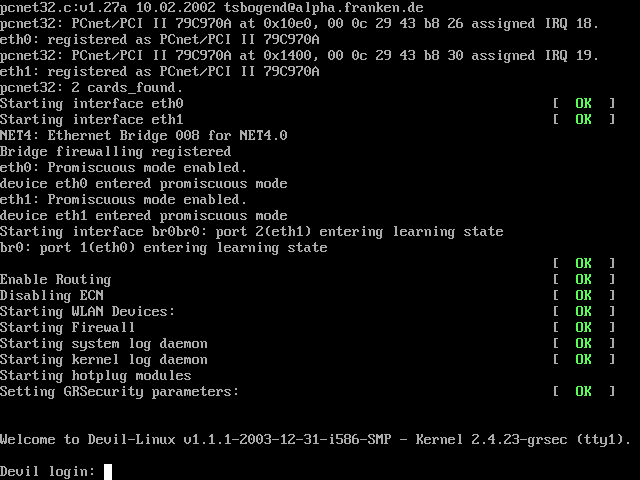
\includegraphics[height=2.4cm]{console-login-screenshot}
      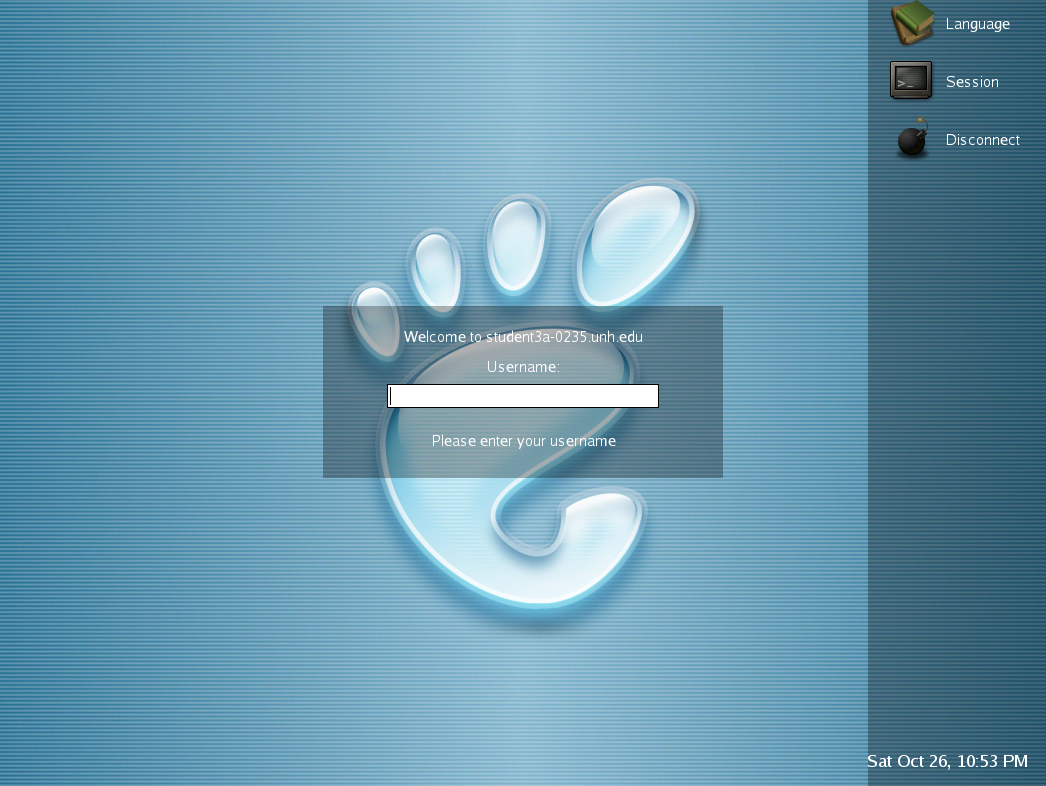
\includegraphics[height=2.4cm]{gdm-login-screenshot}
      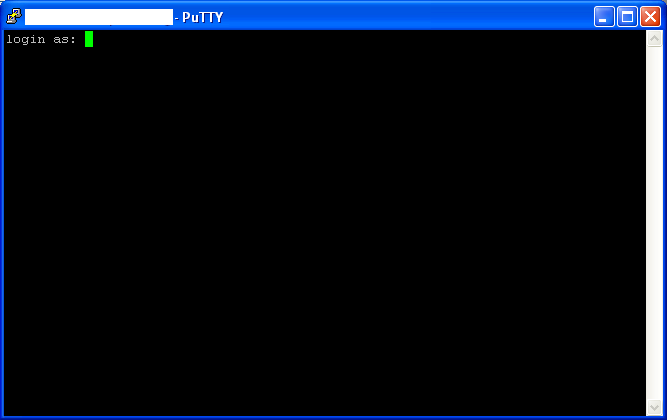
\includegraphics[height=2.4cm]{putty-login-screenshot}
    \end{block}

    \begin{block}<3->{Виды сессий}
      \begin{itemize}
        \item локальные и удалённые (сетевые)
        \item текстовые и графические
      \end{itemize}
    \end{block}

  \end{center}

\end{frame}

\begin{frame}[fragile]
  \frametitle{Входим удалённо. SSH. Secure Shell.}

    Протокол удалённой работы по сети для Linux.

    Много реализаций клиентов и серверов.
    \pause

    \emph{Как может выглядеть:}
    \newline
    \fbox{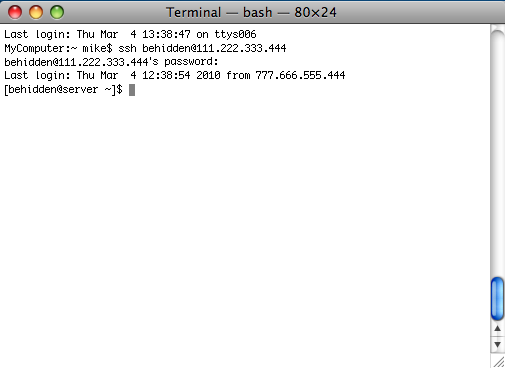
\includegraphics[height=3.5cm]{console-ssh-screenshot}}
    \emph{ }
    \fbox{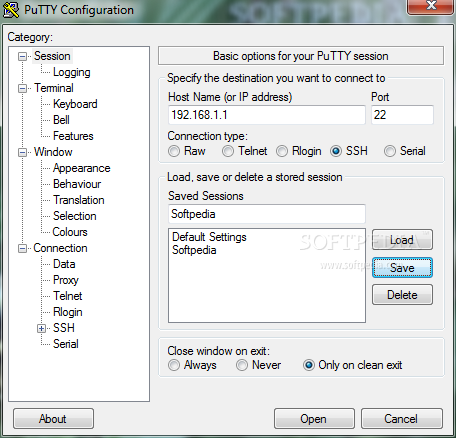
\includegraphics[height=3.5cm]{putty-config-screenshot}}

\end{frame}

\begin{frame}[fragile]
  \frametitle{SSH address}

\begin{block}{Access parameters}
    IP address: 192.168.10.10 \par
    Username: root, val, user \par
    Port: 22 default or any \par
\end{block}
    Full path: root@192.168.10.10:22
\end{frame}

\begin{frame}
  \frametitle{Выход из матрицы}

  \begin{center}
    
\includegraphics[height=5.0cm]{matrix-screenshot}
    \pause
    \newline
    \begin{itemize}
      \item Команда \emph{exit}, команда shell \emph{logout}
      \item Hotkey \emph{Ctrl+d}
      \item Закрыть клиент
    \end{itemize}
  \end{center}

\end{frame}
